\documentclass{llncs}
\usepackage[utf8]{inputenc}
\usepackage{verbatim}
\usepackage{multicol}
\usepackage{llncsdoc}
\usepackage{amsmath}
\usepackage{amsfonts}
\usepackage{amssymb}
\usepackage{graphicx}
\usepackage{lmodern}
\usepackage{calc}
\usepackage{enumitem}
\usepackage{algpseudocode}
\usepackage{algorithm}
\usepackage{algorithmicx}

\algsetblockdefx[IfContinue]{IfContinue}{IfContinue}
{0}{0pt}
[0]{}
[1]{\textbf{if} #1 \textbf{continue}}

\algrenewcommand\algorithmicrequire{%
  \makebox[\widthof{\textbf{Output:}}][l]{\textbf{Input:}}}
  
 \algrenewcommand\algorithmicensure{%
  \textbf{Output:}}

\usepackage{color}
\usepackage{gnuplottex}
\usepackage{subcaption}
\usepackage{microtype}
\usepackage[normalem]{ulem}
\captionsetup{compatibility=false}
\usepackage{tikz}
\usetikzlibrary{trees,automata,positioning}
\usepackage{booktabs}
\usepackage{gnuplottex}
\usepackage{xparse}
\usepackage{epstopdf}
% For scaling gnuplottex
\ExplSyntaxOn
\DeclareExpandableDocumentCommand{\convertlen}{ O{cm} m }
 {
  \dim_to_unit:nn { #2 } { 1 #1 } cm
 }
\ExplSyntaxOff

%% For lattice figure
% Set the overall layout of the tree
\tikzstyle{level 1}=[level distance=3.0cm, sibling distance=0.6cm]
\tikzstyle{level 2}=[level distance=3.5cm, sibling distance=0.6cm]
\tikzstyle{level 3}=[level distance=3.5cm, sibling distance=0.6cm]

% Define styles for bags and leafs
\tikzstyle{l1} = [rectangle, text width=5em, text centered]
\tikzstyle{l2} = [rectangle, text width=5em, text centered]
\tikzstyle{l3} = [rectangle, text width=5em, text centered]

% only when using asmthm
%\newtheorem{definition}{Definition}
%\newtheorem{theorem}{Theorem}

\author{Micky Faas \and Matthijs van Leeuwen}
\title{VOUW: Geometric Pattern Mining using the MDL Principle}
\institute{Leiden Institute for Advances Computer Science}
\begin{document}

\section{Introduction}

Frequent pattern mining is the subfield of data mining that aims to find and extract recurring substructures as a means of data analytics. These patterns can be any kind of datastructure, for example item sets (transactions), graphs (networks) and sequences (in time). So far, little research has been done in applying pattern mining to raster-based, tabular data or matrices. Patterns in these types of data can be more complex as elements cannot only coincide, but their geometric relation is also important. As the first contribution of this paper, we introduce exactly this problem, that we will call \textbf{geometric pattern mining} and formally introduce notation and theoretical constructions for this problem. Potential applications include analysis of (satellite) imagery, texture recognition and clustering of matrices.

\begin{figure}[b]
\centering
\begin{subfigure}[t]{0.35\textwidth}
\centering
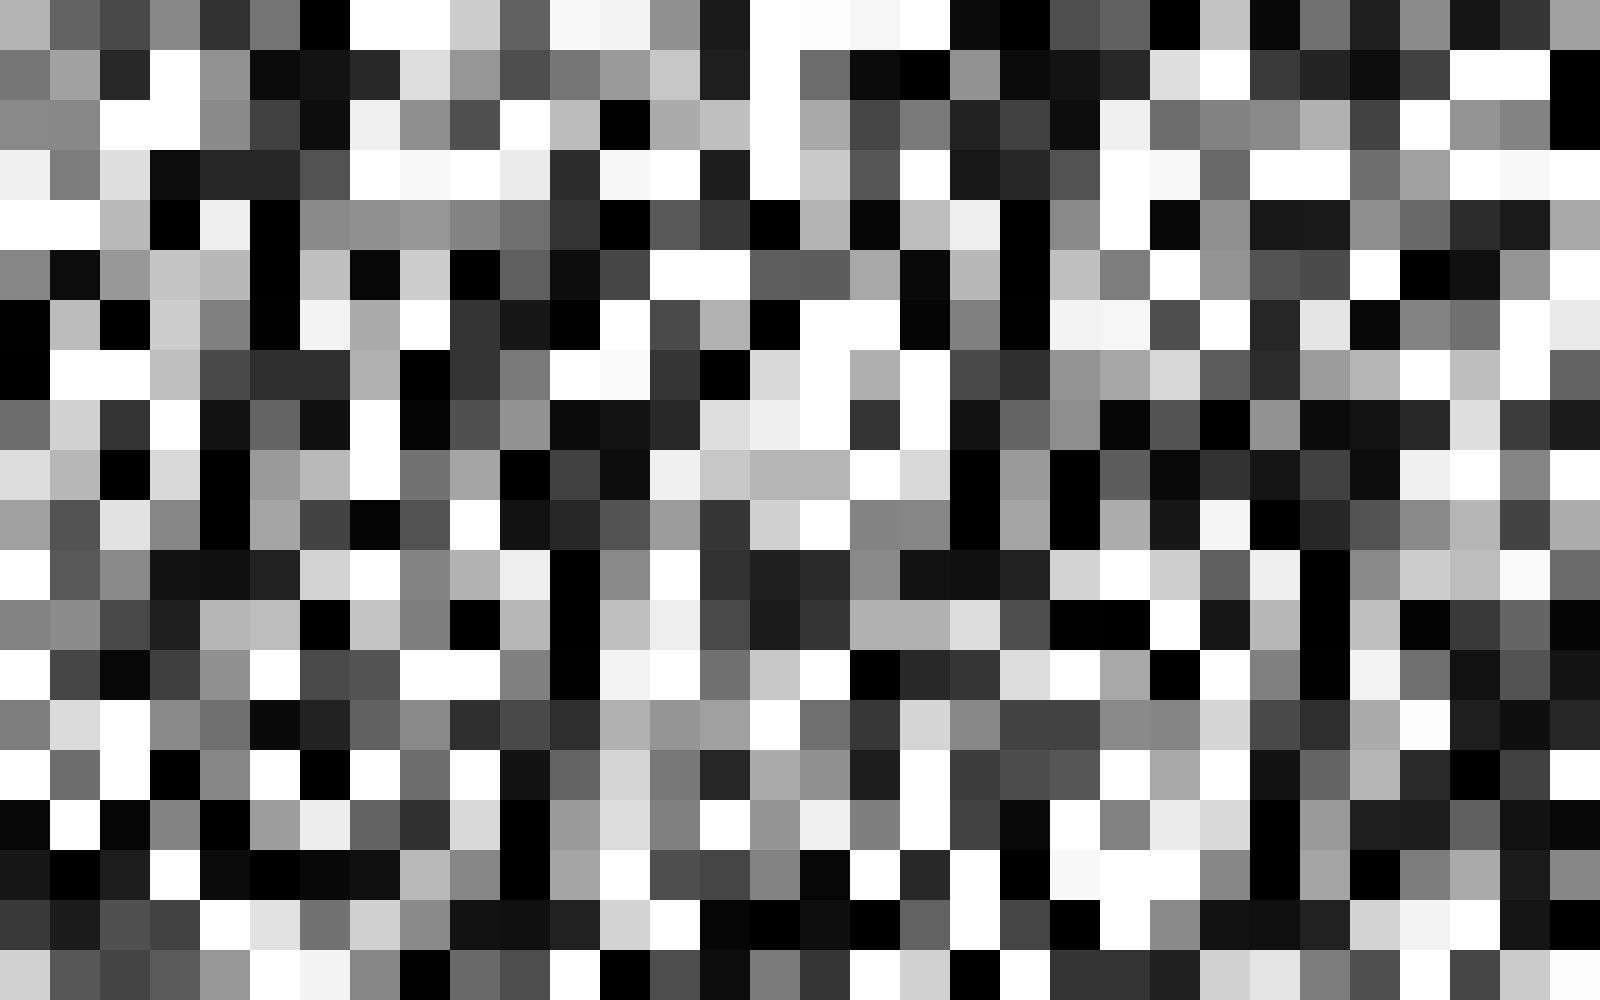
\includegraphics[scale=.25]{img/Garamond-I_cropped.png}
\caption{$32\times 24$ noise `matrix'}
\label{fig-example1a}
\end{subfigure}%
~
\begin{subfigure}[t]{0.20\textwidth}
\centering
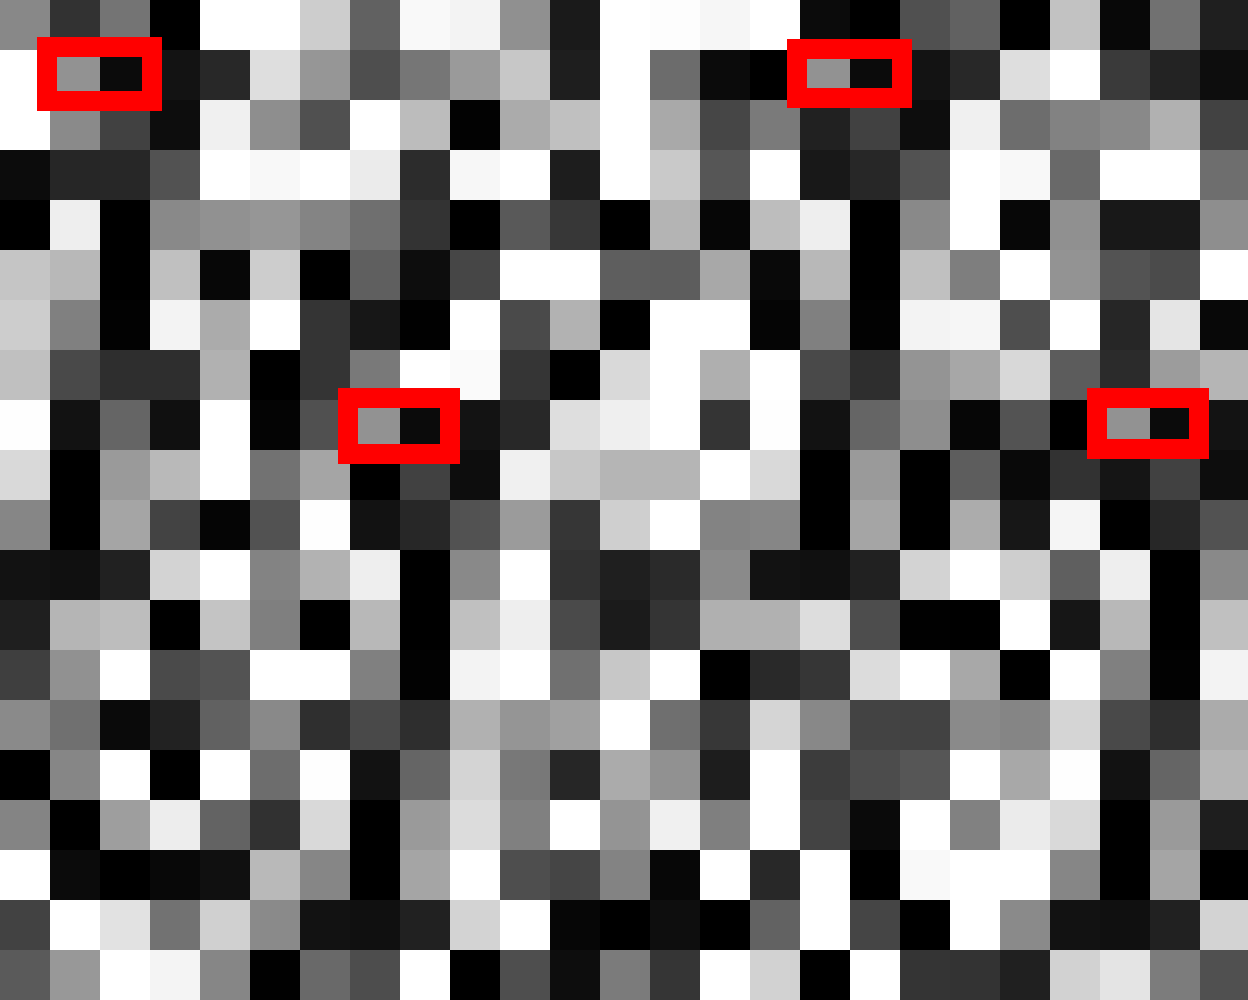
\includegraphics[scale=.25]{img/Garamond-I-highlight_cropped.png}
\caption{Pair $(146,11)$}
\label{fig-example1b}
\end{subfigure}%
~
\begin{subfigure}[t]{0.37\textwidth}
\centering
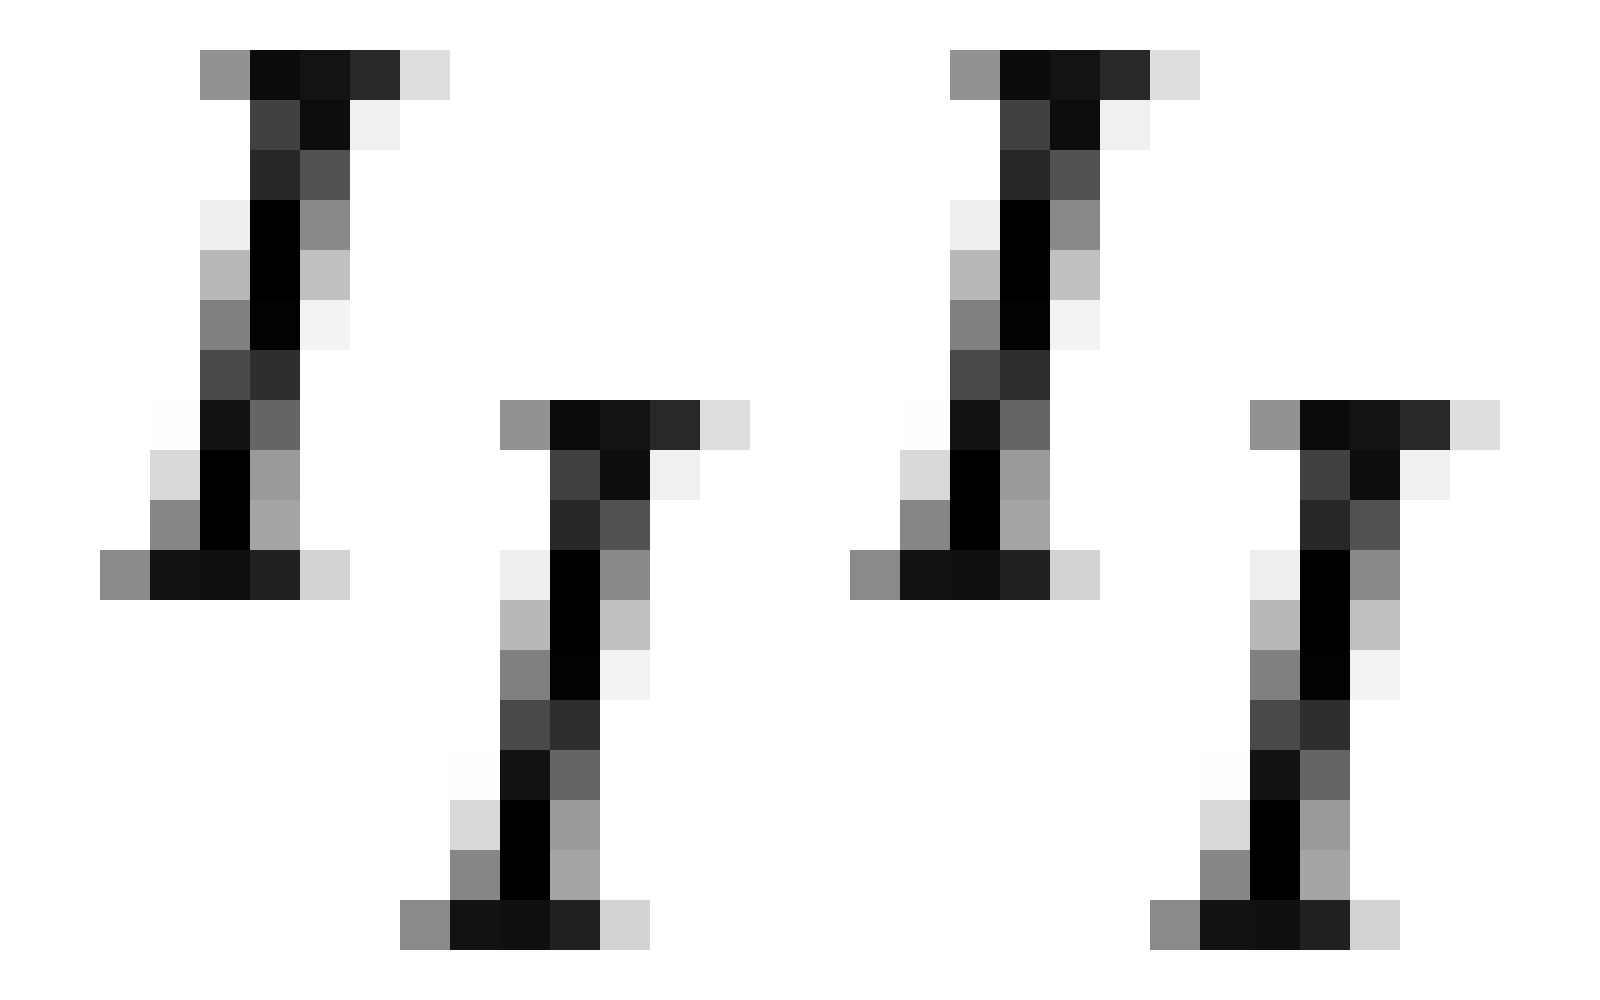
\includegraphics[scale=.25]{img/Garamond-I-clean_cropped.png}
\caption{Pattern `I' occurs four times.}
\label{fig-example1c}
\end{subfigure}%
\caption{Brief example of geometric pattern mining}
\end{figure}  

\subsubsection{Geometric Pattern Mining}

Geometric pattern mining is the problem of finding recurring local structure or \textbf{patterns} in matrices. It is different from graph mining, as a matrix is more rigid and each element has a fixed degree of connectedness/adjacency. It is also unrelated to linear algebra, other then using the term `matrix' and a comparable style of notation. Furthermore in this context, matrix elements can only be discrete, rows and columns have a fixed ordering and the semantics of a value is position-independent. Although the concept applies to any number of dimensions, we will limit the scope to two dimensional data from here on.

The problem of geometric pattern mining can roughly be divided into three classes. The first class consists of three subclasses: finding identical patterns in (1a) an otherwise empty (sparse) matrix, (1b) differently distributed noise and (1c) similarly distributed noise. The second class contains the same subclasses but adds that the patterns can also be overlaid with noise and are therefore not identical. The third class is also a continuation of the first class and requires that the patterns are identical after some optional transformation (such as mirror, inverse, rotate, etc.). These classes also represent an increasing difficulty level and serves as a rough benchmark for the performance of an algorithm. 

Let us demonstrate the problem of geometric pattern mining with a brief example. Figure \ref{fig-example1a} shows a $32 \times 24$ grayscale `matrix' filled with noise on the interval $[0;255]$. If we look at all horizontal pairs of elements, we find that the pair $(146,11)$ is, among others, statistically more prevalent than `random noise' suggests. If we would continue to try all combinations of elements that `stand out' from the background noise, Figure \ref{fig-example1c} shows that we will eventually find four copies of the letter `I' set in 16 point Garamond Italic.
% Figure \ref{fig-example1b} highlights the locations where these pairs occur.

The 35 elements that make up a single `I' in the example form a \textbf{pattern}. We can use this pattern to describe the matrix in an other way than `768 unrelated values'. For example, we could describe it as 628 unrelated values plus pattern `I' at locations $(5,4), (11,11), (20,3), (25,10)$, separating the structure from the accidental (noise) data. Since this requires less storage space than before, we have compressed the data. At the same time we have learned something about this data, namely that it contains four `hidden I's. 

%The example in the previous section belongs to class 1b: the structures are surrounded by noise, but their distribution clearly stands out.

%Although we could intuitively solve the example, in reality it is much more complex. Is the `I' the best pattern we can find (and why), are there any more patterns and, most important, how do we find it (quickly) in an unknown and/or much larger dataset? After formally defining these problems and their contexts we will introduce VOUW, a novel geometric pattern mining algorithm based on the MDL principle. 

\subsubsection{Datamining by Compression}
 
In recent years, a class of algorithms utilizing the \emph{Minimum Description Length (MDL) principle} \cite{rissanenmdl,grunwaldmdl} have become more and more common in the field of explanatory data analysis. Examples of such approaches include Krimp \cite{krimp} or more recently Classy \cite{classy}. The  MDL principle was first described by Rissanen in 1987 \cite{rissanenmdl} as a practical implementation of Kolmogorov Complexity \cite{kolmogorov}. Central to MDL is the notion that `learning' can be thought of as `finding regularity' and that regularity itself is a property of data that is exploited by \emph{compressing} said data. Therefore by compressing a dataset, we actually learn its structure --- how regular it is, where this regularity occurs, what it looks like --- at the same time. %Indeed MDL postulates that the most optimal compression (minimal description) of a given dataset provides the best description of that data. 

The problem that MDL solves first and foremost, is that of \emph{model selection}: given a multitude of explanations (models), select the one that fits the data best. In addition to this, MDL has also been demonstrated to be very effective in materialization of a specific model given the data. In this case, the model is predetermined and we want to find the parameters to fit the data. A similar problem class is solved in pattern mining: here the `parameters' are the discrete building blocks that make up patterns in the data. We will specifically look at a variant of MDL called two-part MDL. As the second contribution of this paper, we present a geometric pattern mining algorithm that (1) is precise, (2) requires no parameters and (3) is tolerant to noise in the data, based on two-part MDL.
 
\end{document}
